\documentclass[10pt]{beamer}

\usepackage[utf8]{inputenc}
\usepackage[T1]{fontenc}
\usetheme[progressbar=frametitle]{metropolis}
\usepackage{appendixnumberbeamer}

\usepackage{booktabs}
\usepackage[scale=2]{ccicons}

\usepackage{pgfplots}
\usepgfplotslibrary{dateplot}

\usepackage{xspace}
\newcommand{\themename}{\textbf{\textsc{metropolis}}\xspace}

\usepackage{tikz}
\usetikzlibrary{positioning, arrows, shapes}
\usetikzlibrary{shapes}
% Define box and box title style
\tikzstyle{mybox} = [draw, very thick, rectangle, inner sep=10pt, inner ysep=20pt, fill=black, text=white, minimum width=\textwidth, minimum height=2cm]

\tikzstyle{redRectangle} = [
    rectangle,
    draw,
    fill=red!20,
    node distance=0.85 cm,
    text width=7 em,
    text centered,
    rounded corners,
    minimum height=4 em,
    minimum width=3 cm,
    thick
    ]
    \tikzstyle{blueRectangle} = [
    rectangle,
    draw,
    fill=blue!20,
    node distance=1.5 cm,
    text width=7 em,
    text centered,
    rounded corners,
    minimum height=4 em,
    minimum width=3 cm,
    thick
    ]
    \tikzstyle{yellowRectangle} = [
    rectangle,
    draw,
    fill=yellow!20,
    node distance=1.5 cm,
    text width=7 em,
    text centered,
    rounded corners,
    minimum height=4 em,
    minimum width=3 cm,
    thick
]
\tikzstyle{empty} = []

\title{Como contar uma história com seu código}
\subtitle{Programação Literária com Notebooks}
% \date{\today}
\date{TDC Floripa 2017}
\author{Melissa Weber Mendonça}
\institute{UFSC}
\titlegraphic{\hfill
\includegraphics[height=1.5cm]{imagens/brasao_UFSC.png}}

\begin{document}

\maketitle

\begin{frame}
  \frametitle{Motivação}
  \begin{center}
    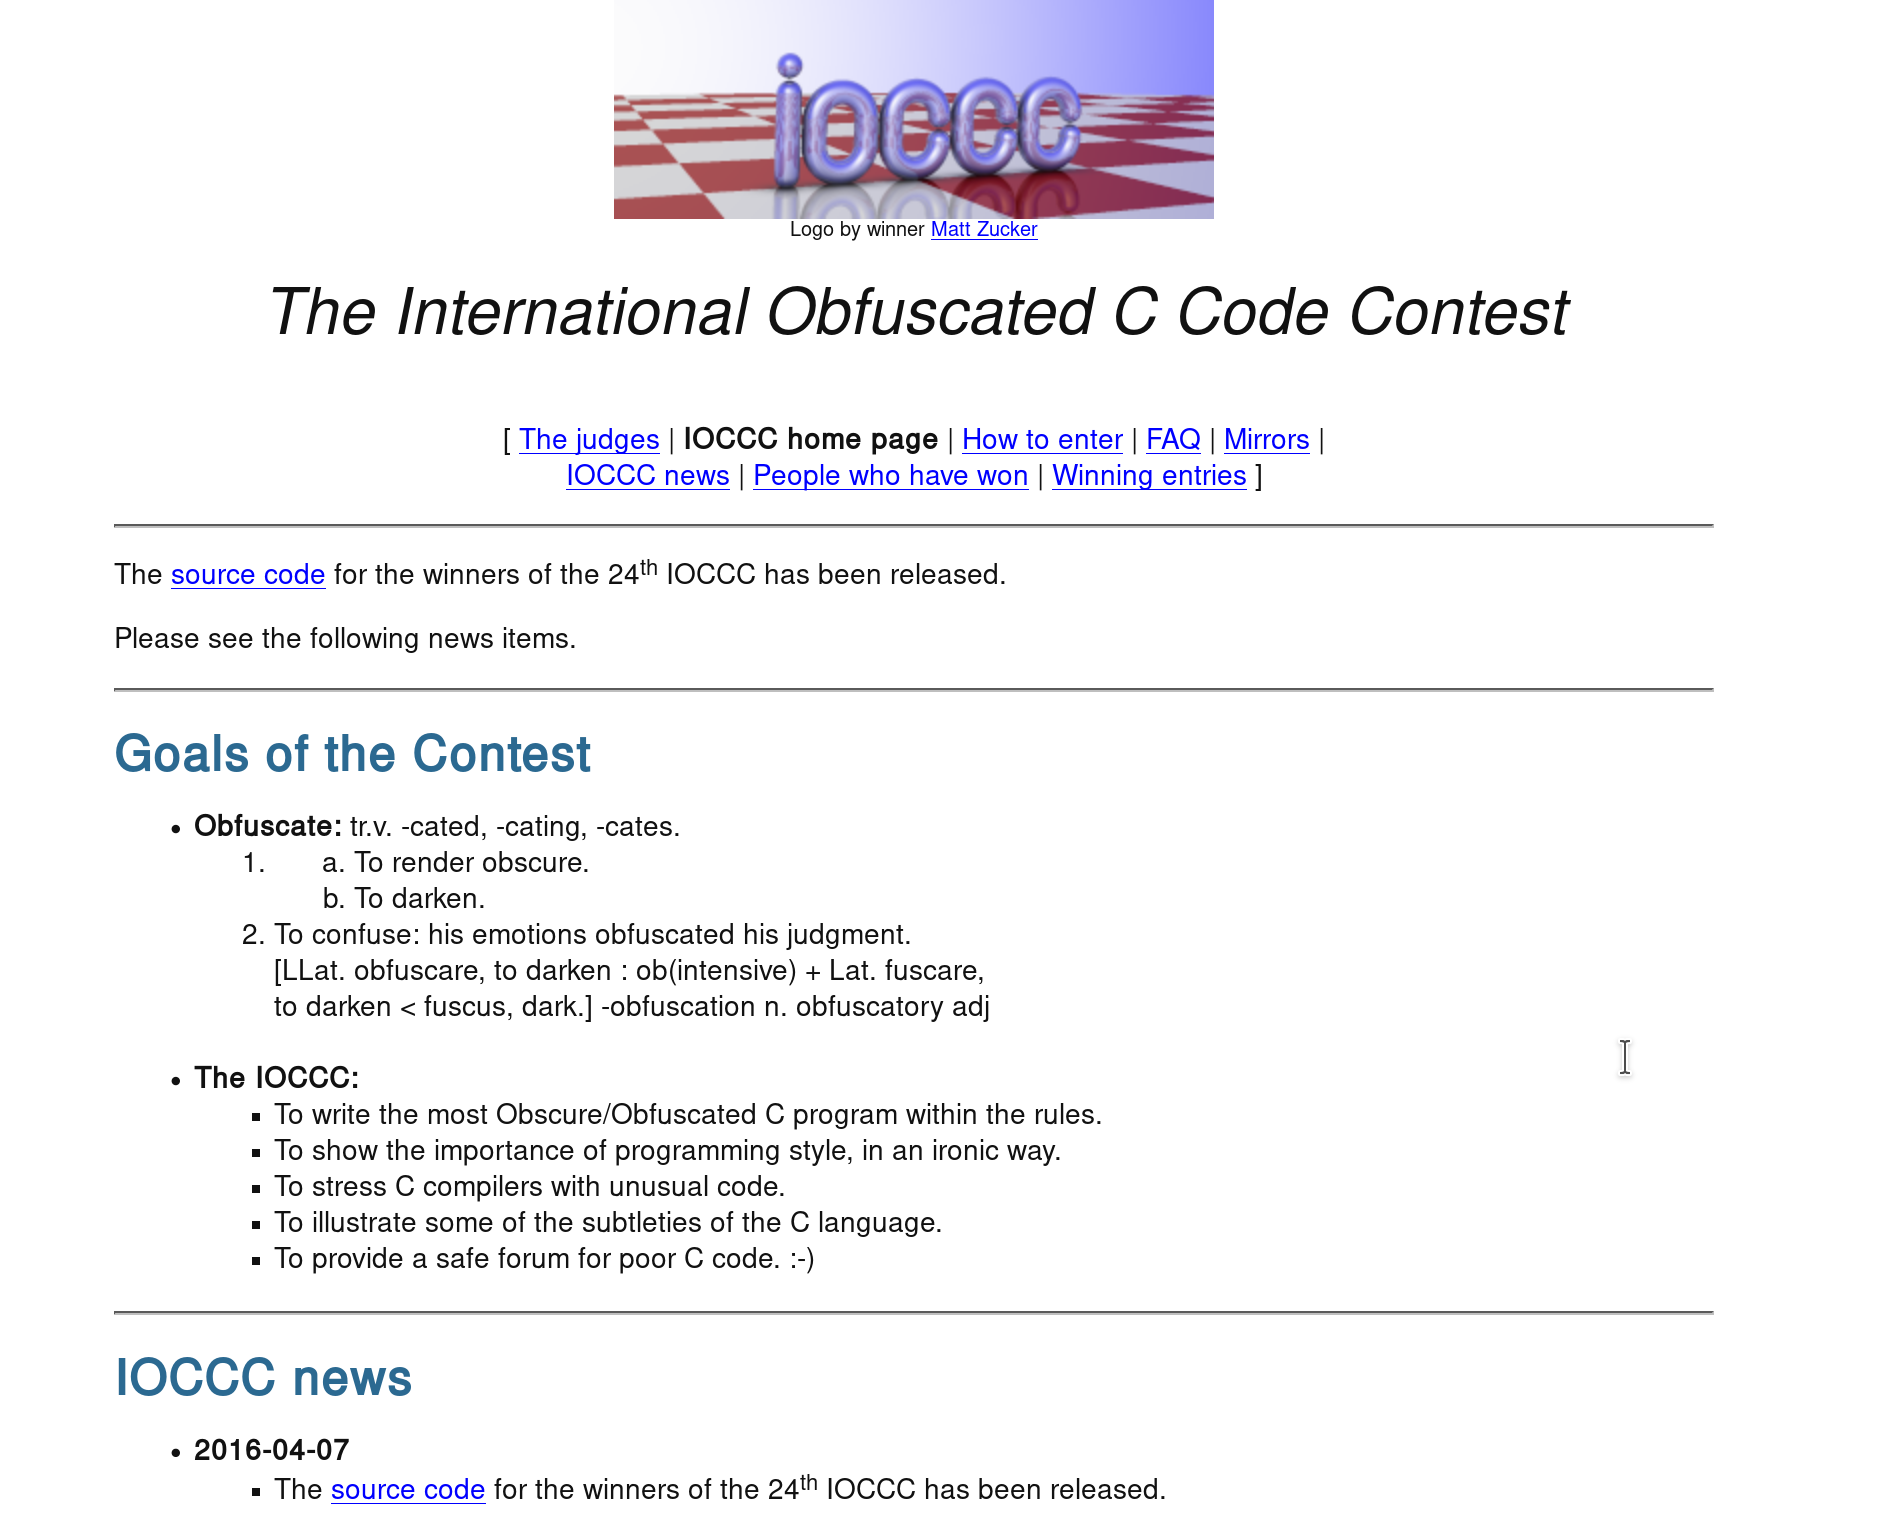
\includegraphics[width=0.9\textwidth]{imagens/obfuscated.png}
  \end{center}
\end{frame}

\begin{frame}
  \frametitle{Motivação}
  \begin{center}
  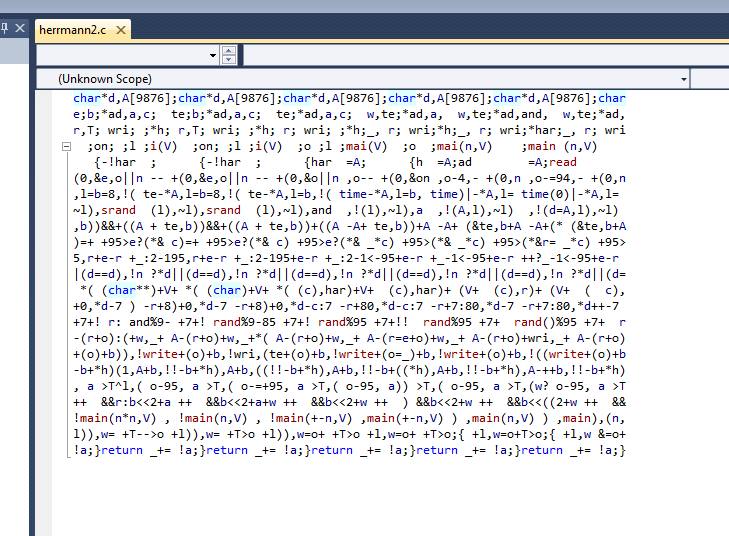
\includegraphics[width=0.9\textwidth]{imagens/ioccc.png}
  \end{center}
\end{frame}

\begin{frame}
  \frametitle{Literate Programming}
  \begin{itemize}
  \item Linguagem natural + macros/código
  \item \emph{Compilável}
  \item Lógica da máquina v. Lógica humana
  \end{itemize}
  \begin{columns}
    \column{5cm}
    \begin{center}
      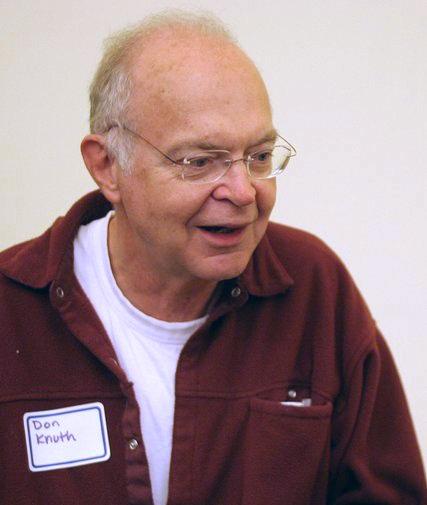
\includegraphics[width=3.4cm]{imagens/knuth.jpg}\\
      Don Knuth (1981)
    \end{center}
    \column{5cm}
    \begin{center}
      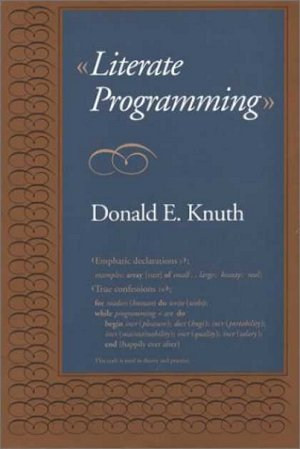
\includegraphics[width=3cm]{imagens/Literate_Programming_book_cover.jpg}
    \end{center}
  \end{columns}
\end{frame}

\begin{frame}
  \frametitle{Linguagem natural v. Linguagem de máquina}
%     Instead of imagining that our main task is to instruct a computer what to do, let us concentrate rather on explaining to human beings what we want a computer to do.
  % Overall, web is combination of two languages: 1) Document formatting Language 2) Programming language. Although Pascal and TeX is the most commonly used combination for Literate programming, documentation language may include TeX, Scribe, Troff while programming languages can be Pascal, A, ALGOL, LISP, COBOL, FORTRAN, APL, C, etc.[1]
  \begin{itemize}
  \item Código como literatura
  \item Descrever a lógica explicitamente
  \item Documentação orgânica
  \item \alert{Pesquisa e reproducibilidade} 
  \begin{itemize}
  	\item \emph{provenance}
    \item \emph{scientific workflow}
  \end{itemize}
  \end{itemize}
\end{frame}

\begin{frame}[fragile]
  \frametitle{Literate Programming: WEB}
  WEB foi o primeiro sistema de LP [https://en.wikipedia.org/wiki/WEB]
  \begin{center}
    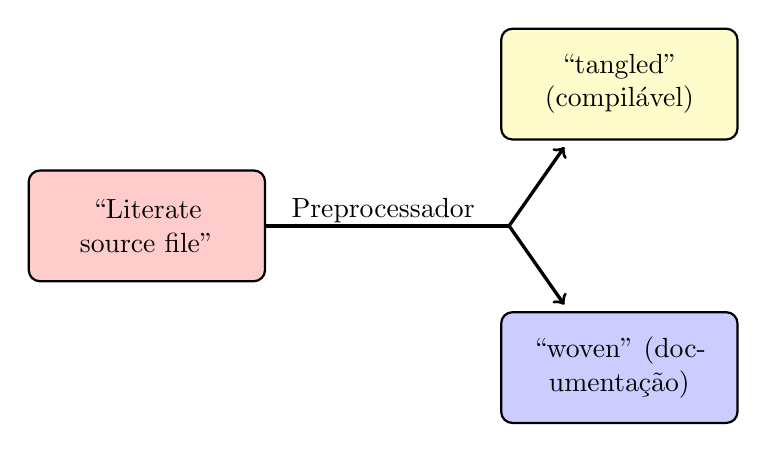
\begin{tikzpicture}
      \node[redRectangle] at (0,0) (source) {``Literate source file''};
      \draw[very thick] (source.east) -- (4.6,0);
      \node[] at (3,0.2) {Preprocessador};
      \draw[very thick, ->] (4.6,0) -- (5.3,1);
      \draw[very thick, ->] (4.6,0) -- (5.3,-1);
      \node[yellowRectangle] at (6,1.8) {``tangled'' (compilável)};
      \node[blueRectangle] at (6,-1.8) {``woven'' (documentação)};
    \end{tikzpicture}
  \end{center}

  \begin{center}
    \href{https://github.com/zyedidia/Literate/blob/master/examples/wc.lit}{\beamergotobutton{wc.lit}}
  \end{center}
\end{frame}

\begin{frame}
  \frametitle{Implementações}
  \begin{itemize}
  \item WEB \textemdash\ Pascal + \TeX\ (Knuth) 
  \item CWEB \textemdash\ C + \TeX\ (Knuth e Silvio Levy)
  \item Sweave \textemdash\ R + \TeX
  \item knitr \textemdash\ R+\TeX
  \item noweb \textemdash\ Linguagem? + Formato? (HTML)
  \item iJulia
  \item Pweave \textemdash\ Python + Formato? (Pandoc)
  \item \alert{iPython/Notebooks}
  \end{itemize}
\end{frame}

\begin{frame}
  \frametitle{O que não é Literate Programming}
  \begin{itemize}
  \item Código bem documentado
  \item Relatórios incluindo código e texto 
  \item Documentação automática
  \item Notebooks escritos de maneira "tradicional" (código colocado no notebook ao invés de uma IDE)
  \end{itemize}
\end{frame}

\begin{frame}
  \frametitle{}
  \begin{center}
    \begin{block}
      {Donald Knuth. "Literate Programming (1984)" \footnote{in Literate Programming. CSLI, 1992, pg. 99.}}
      Let us change our traditional attitude to the construction of programs: Instead of imagining that our main task is to instruct a computer what to do, let us concentrate rather on explaining to human beings what we want a computer to do.
      
      The practitioner of literate programming can be regarded as an essayist, whose main concern is with exposition and excellence of style. Such an author, with thesaurus in hand, chooses the names of variables carefully and explains what each variable means.
    \end{block}
  \end{center}
\end{frame}

\begin{frame}
  \frametitle{Tradução Livre}
  \begin{center}
    \begin{block}
      {Donald Knuth. "Literate Programming (1984)" }
      Vamos mudar nossa atitude tradicional em relação à construção de programas: Ao invés de imaginarmos que nossa tarefa principal é instruir o computador, \textbf{vamos nos concentrar em explicar para seres humanos o que queremos que o computador faça}.
      
      O praticante de programação literária pode ser visto como um ensaísta, cuja preocupação principal é a excelência no estilo e na exposição. Um autor assim, com dicionário em mãos, escolhe os nomes das suas variáveis com cuidado e explica o que cada uma delas significa.
    \end{block}
  \end{center}
\end{frame}

\begin{frame}[fragile]
  \frametitle{Exemplo}
     \begin{center}
      \begin{minipage}{0.7\textwidth}
      \begin{block}{}
         \begin{center}
              \verb+IDEB.ipynb+
         \end{center}
      \end{block}
    \end{minipage}
   \end{center}
   \vfill
   Algumas ferramentas úteis:
   \begin{itemize}
   \item \LaTeX
   \item Pandoc
   \item nbextensions: codefolding, initialization cell, limit output
   \item Preprocessors e templates para notebooks
   \end{itemize}
\end{frame}

\begin{frame}[fragile]
   \frametitle{}
   \begin{center}
      \begin{minipage}{0.7\textwidth}
      \begin{block}{}
         \begin{center}
            \href{https://github.com/melissawm}{github.com/melissawm}\\
            \href{http://www.mtm.ufsc.br/~melissa}{mtm.ufsc.br/\~{}melissa}
         \end{center}
      \end{block}
    \end{minipage}
    \vfill

    Obrigada!
   \end{center}
\end{frame}

\begin{frame}[allowframebreaks, fragile]{Material de Apoio}

	\begin{itemize}
	\item Bons notebooks:
    \begin{itemize}
    \item \href{http://nbviewer.jupyter.org/gist/rpmuller/5920182}{A Crash Course in Python for Scientists (Rick Muller)}
    \item \href{http://nbviewer.jupyter.org/github/jrjohansson/scientific-python-lectures/blob/master/Lecture-4-Matplotlib.ipynb}{matplotlib \textemdash\ 2D and 3D plotting in Python (J.R. Johansson)}
    \end{itemize}
    \item Notebooks ruins:
    \begin{itemize}
    \item \href{http://nbviewer.jupyter.org/github/facebook/iTorch/blob/master/iTorch_Demo.ipynb}{iTorch Demo (??)}
    \item \href{http://nbviewer.jupyter.org/github/bokeh/bokeh-notebooks/blob/master/gallery/texas.ipynb}{Exemplo Bokeh}
    \end{itemize}
    \end{itemize}
    % Link interessante!
    %http://blog.juliusschulz.de/blog/ultimate-ipython-notebook
\end{frame}
\end{document}